\documentclass[a4paper,12pt]{article}
\usepackage{algorithm} 
\usepackage{algpseudocode} 
\usepackage[a4paper, total={7in, 10in}]{geometry}
\usepackage{graphicx}

\author{Michalis Christou}
\title{Parallel vs Serial Fault Simulator}
\begin{document}
\maketitle

\section*{Introduction}
The purpose of this project is to write a fault simulator in C++ that supports both parallel and serial modes of operation. The goal is to examine the speedup of the parallel implementation compared to the serial version as well as compare any potential performance increases that might occur with or without fault dropping in both cases.


\section*{Background}
\subsection*{Single Stuck at Fault Model}
Faults in circuits can be modeled in many ways. The model that was used for the purposes of this project was the single stuck at fault model. In this case the circuit, which is a gate level netlist, has only one faulty line that is either stuck permanently at $1$ or $0$ and the fault can be at an input or output of a gate. The number of possible fault sites in a given netlist is $\# PI + \#GATES + \#(fanout branches)$ and subsequently since a fault site has 2 potential faults, the number of possible faults in a circuit is $2 \cdot \#(fault sites)$. 

\subsection*{Fault Equivalence}
Despite a circuit having a maximum number of possible stuck at faults, using some mechanisms we can choose a subset of these faults and if we are able to detect these it means that we can also detect the ones we skipped. For example, fault equivalence means that two faults $f_1, f_2$ are equivalent if all tests that detect $f_1$ also detect $f_2$ and vice versa. This means that if we are able to detect one of the two faults then we know for sure that we can detect the other as well. Thus we can keep only one of these equivalent faults in our list. This is called fault collapsing. The result is a collapsed fault set that contains one fault from each equivalence subset.

\subsection*{Fault Dominance}
The definition of fault dominance is as follows, if all tests of some fault $f_1$ detect another fault $f_2$ then $f_2$ is said to dominate $f_1$. The rule that we use is if fault $f_2$ dominates $f_1$ then $f_2$ is removed from the fault list.

\subsection*{Checkpoint Theorem}
The checkpoint theorem is the result of Fault Equivalence and Fault Dominance. Primary inputs and fanout branches of a combinational circuit are called checkpoints. The theorem suggests that a test set that detects all single stuck at faults on all checkpoints of a combinational circuit also detects all single stuck at faults in that circuit. The checkpoints in a circuit are considered to be primary inputs and fanout branches. This means that if we only consider these fault sites and detect all faults in them, we can also detect all possible stuck at faults in that circuit.

\section*{Fault Simulation}
Fault simulation is done in order to detect possible faults in a Boolean circuit. The algorithm is fairly simple and intuitive. First a set of test vectors is obtained. Then using these test vectors the non-faulty circuit response is computed. Then for each stuck at fault that is considered, the fault is injected in the circuit, the fault output is computed and compared to the normal non-faulty output. If the outputs differ, then the fault can be detected. In this case a detected fault counter is incremented. If fault dropping is enabled, then the stuck at fault is deleted from the set. After this is repeated for all test vectors and all faults in the set the fault coverage is computed which is the number of detected faults divided by the total number of faults considered. 

$$FC = \frac{\#fd}{\#tf}$$

The pseudo-code for the serial algorithm is depicted below.

\begin{algorithm}
	\caption{Serial Fault Simulation} 
	\begin{algorithmic}[1]
		\State $\#fd = 0, \#tf = |F|$
		\For {every test $t \in T$}
			\State $Rt = $ true\_value\_simulation($t,C$)
			\For {every fault $f \in F$}
					\State inject\_fault($C,f$)
					\State $Rf = $ fault\_simulation($C,f$)
				\If {$Rt \neq Rf$}
					\State $\#rf++$
					\State $F = $ drop\_fault($t,F$)
				\EndIf	
			\EndFor
		\EndFor
					\State \textbf{return} $FC = $ compute\_fault\_coverage($\#fd,\#tf$)
	\end{algorithmic} 
\end{algorithm}


\clearpage

\section*{Implementation}
This section is dedicated to explaining the details and inner workings of the C++ implementation. The code is designed to parse \texttt{.bench} files that represent gate level netlists as well as test vectors of different formats. Then the code generates all faults according to the Checkpoint Theorem. Depending on the user input the program either runs the serial algorithm or parallel with or without fault dropping. By utilizing bash scripts the simulator can be used via it's command line arguments. The following diagram shows how a collection of bash scripts and the simulator program work together to produce the necessary results.

\begin{figure}[h]  
  \centering
    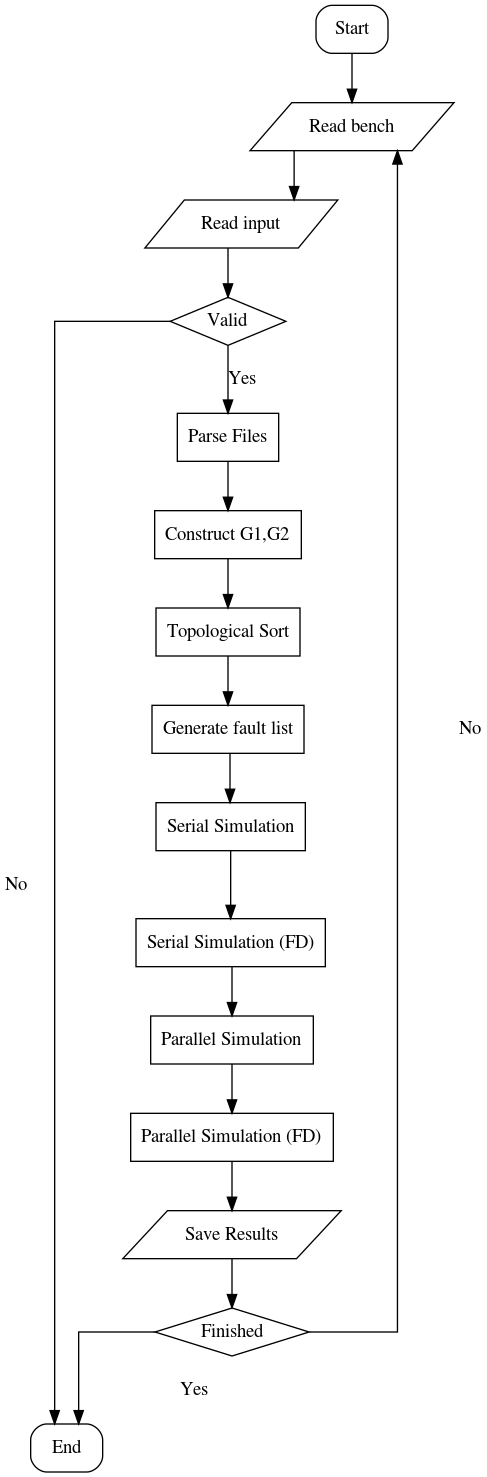
\includegraphics[width=0.35\textwidth]{Diagram.png}
	%\caption{A picture of a gull.}
\end{figure}

\clearpage
\subsection*{Netlist Representation}
The netlist is internally represented as a DAG (Directed Acyclic Graph). Specifically, since the purpose of the program is to simulate faults, the graph model that was chosen was $G_2$. This model uses one graph node per circuit line and one edge per pair of gates/fanout stems with direct connection, in order to explicitly represent fanout stems. This is necessary in this case because faults could happen in any circuit line thus explicit representation of every line is needed. The data structure used in this case was a $1-D$ array with linked lists, since generally speaking, Boolean circuits are sparse thus more memory is saved compared to using a $2-D$ array. 

\subsection*{Parallelizing Fault Simulation}
When parallelizing algorithms a lot of factors have to be considered. Data dependencies is one aspect that leads to race conditions which in turn, leads to unpredictable code behavior. In this case, the most important part of parallelizing the algorithm is to ensure that no data dependencies or race conditions would occur. In this case this was achieved easily by splitting the work in equal chunks to $N$ threads. Since each iteration is almost fully independent splitting the workflow to any number of threads is trivial once the serial algorithm is implemented. The workflow is split as follows: Each thread receives a subset of the test vector set, then independently workes on identifying all faults that were previously generated with the checkpoint theorem and stored in a global variable. When using fault dropping, threads that detect faults need to modify a global variable (that stores faults) in order to save time for other threads. To ensure that threads would not interfere with one another the global data structure was protected with a mutex since it was part of a critical region, but this was only a problem when using fault dropping. Without fault dropping each thread can work fully independent from any other one.

\clearpage


\section*{CLI Arguments}

One of the aspects of this project is to run many simulations with different input files and settings. Due to this necessity, the simulator is implemented to use command line arguments that control it's functionality. Below a list of all command line options is shown and each argument is explained with example usage.
\\\\
When the simulator is used in the following fashion it just uses the benchmark file and corresponding input file given by the user, computes the fault coverage in serial mode and prints useful statistics in stdout including the fault coverage. This is the most basic usage. 
\\\\ \texttt{./simulator -C <benchmark\_path> -I <test\_path> -S} \\\\
The \texttt{-S} parameter can be combined with the \texttt{-T <[s],[ms],[us],[ns]>} argument in order to get the total run-time of the program as well as the netlist stats in stdout. The user can also choose the time unit. The next example prints netlist stats as well as the total runtime in seconds.
\\\\ \texttt{./simulator -C <benchmark\_path> -I <test\_path> -S -T s} \\\\
Apart from computing the fault coverage the simulator can output the test vector that detected faults in a txt file via the \texttt{-H} argument. The usage in this case is as expected. 
\\\\ \texttt{./simulator -C <benchmark\_path> -I <test\_path> -H} \\\\
The next argument tells the simulator in which mode to run (serial or parallel) and to how many threads to allocate the work. If no number of theads is given then the simulator chooses the maximum number of concurrent threads supported by the CPU. In this instance the simulator will run in parallel on 8 threads.
\\\\ \texttt{./simulator -C <benchmark\_path> -I <test\_path> -P 8} \\\\
Another useful argument is \texttt{-D} which enables fault dropping mode. This can dramatically decrease the simulation time while still giving out correct results. It's an optimization step that is useful for comparing test vector quality.
\\\\ \texttt{./simulator -C <benchmark\_path> -I <test\_path> -D} \\\\
\clearpage
An argument that doesn't change the functionality of the simulator but comes in handy when working wit large netlists is the \texttt{-B} option. This option gives user feedback about the progress of the simulator, estimated execution time and how many input patterns per second are applied to the netlist. The argument is used like so: 
\\\\ \texttt{./simulator -C <benchmark\_path> -I <test\_path> -B} \\\\
For example, by running the simulator with the following arguments:
\\\\ \texttt{./simulator -C s5378.bench -I s5378.vec -B} \\\\
We get the following output:
\\\\ \texttt{[100 P/s][total 0][0\% done][100\% in 75 min]} \\\\
But when running the simulator in parallel:
\\\\ \texttt{./simulator -C s5378.bench -I s5378.vec -B -P 8} \\\\
We get the following:
\\\\\texttt{[500 P/s][total 0][0\% done][100\% in 15 min]}\\\\
This is great for user feedback as well as a quick first look of how well the work is parallelized. I this case we can clearly see that when using the parallel mode, the simulator will finish approximately 5 times faster. Do note that all arguments can be combined. In the following example the simulator will output stats as well as total run-time in stdout when it's done, use fault dropping and run in parallel on 8 concurrent threads.
\\\\ \texttt{./simulator -C <benchmark\_path> -I <test\_path> -T s -S -D -P 8} \\\\

\clearpage 

\section*{Netlist Statistics}

The table below shows some useful netlist statistics for all benchmark circuits. The table includes circuit data from both ISCAS85 and ISCAS89 benchmarks.


\begin{center}
\begin{tabular}{||c c c c c c c c c c c||}
\hline
Circuit & Nand & And & Nor & Or& Not & Buff & PI & PO & Paths & KB \\ [0.5ex] 
\hline\hline
s27 & 1 & 1 & 4 & 2 & 2 & 0 & 7 & 4 & 28 & 5 \\ 
\hline
s386 & 0 & 83 & 0 & 35 & 41 & 0 & 13 & 13 & 207 & 77 \\ 
\hline
s510 & 61 & 34 & 55 & 29 & 32 & 0 & 25 & 13 & 369 & 100 \\ 
\hline
s641 & 4 & 90 & 0 & 13 & 272 & 0 & 54 & 42 & 1722 & 130 \\ 
\hline
s838.1 & 57 & 105 & 70 & 56 & 158 & 0 & 66 & 33 & 1714 & 186 \\ 
\hline
s298 & 9 & 31 & 19 & 16 & 44 & 0 & 17 & 20 & 231 & 61 \\ 
\hline
s382 & 30 & 11 & 34 & 24 & 59 & 0 & 24 & 27 & 400 & 78 \\ 
\hline
s400 & 36 & 11 & 34 & 25 & 56 & 0 & 24 & 27 & 448 & 82 \\ 
\hline
s526 & 22 & 56 & 35 & 28 & 52 & 0 & 24 & 27 & 410 & 106 \\ 
\hline
s713 & 28 & 94 & 0 & 17 & 254 & 0 & 54 & 42 & 21812 & 145 \\ 
\hline
s344 & 18 & 44 & 30 & 9 & 59 & 0 & 24 & 17 & 344 & 65 \\ 
\hline
s344.1 & 18 & 44 & 30 & 9 & 59 & 0 & 24 & 17 & 344 & 65 \\ 
\hline
s420.1 & 29 & 49 & 34 & 28 & 78 & 0 & 34 & 17 & 474 & 91 \\ 
\hline
s820 & 54 & 76 & 66 & 60 & 33 & 0 & 23 & 24 & 492 & 163 \\ 
\hline
s953 & 114 & 49 & 112 & 36 & 84 & 0 & 45 & 52 & 1156 & 193 \\ 
\hline
s208.1 & 15 & 21 & 16 & 14 & 38 & 0 & 18 & 9 & 142 & 43 \\ 
\hline
s349 & 19 & 44 & 31 & 10 & 57 & 0 & 24 & 17 & 354 & 66 \\ 
\hline
s444 & 58 & 13 & 34 & 14 & 62 & 0 & 24 & 27 & 535 & 90 \\ 
\hline
s1238 & 125 & 134 & 57 & 112 & 80 & 0 & 32 & 32 & 3559 & 245 \\ 
\hline
s1494 & 0 & 354 & 0 & 204 & 89 & 0 & 14 & 25 & 976 & 293 \\ 
\hline
s5378 & 0 & 0 & 765 & 239 & 1775 & 15 & 214 & 228 & 13542 & 1064 \\ 
\hline
s832 & 54 & 78 & 66 & 64 & 25 & 0 & 23 & 24 & 506 & 165 \\ 
\hline
s1423 & 64 & 197 & 92 & 137 & 167 & 0 & 91 & 79 & 44726 & 289 \\ 
\hline
s1196.1 & 119 & 118 & 50 & 101 & 141 & 0 & 32 & 32 & 3098 & 236 \\ 
\hline
s1488 & 0 & 350 & 0 & 200 & 103 & 0 & 14 & 25 & 962 & 292 \\ 
\hline
s9234 & 528 & 955 & 113 & 431 & 3570 & 0 & 247 & 250 & 244854 & 1823 \\ 
\hline
s13207 & 849 & 1114 & 98 & 512 & 5378 & 0 & 700 & 790 & 1345369 & 2683 \\ 
\hline
s15850 & 968 & 1619 & 151 & 710 & 6324 & 0 & 611 & 684 & 164738046 & 3176 \\ 
\hline
s38417 & 2050 & 4154 & 2279 & 226 & 13470 & 0 & 1664 & 1742 & 1391579 & 7703 \\ 
\hline
s38584 & 2126 & 5516 & 1185 & 2621 & 7805 & 0 & 1464 & 1730 & 1080723 & 7734 \\ 
\hline
s35932 & 7020 & 4032 & 0 & 1152 & 3861 & 0 & 1763 & 2048 & 197141 & 7249 \\ 
\hline
c17 & 6 & 0 & 0 & 0 & 0 & 0 & 5 & 2 & 11 & 3 \\ 
\hline
c880 & 87 & 117 & 61 & 29 & 63 & 26 & 60 & 26 & 8642 & 174 \\ 
\hline
c1355 & 416 & 56 & 0 & 2 & 40 & 32 & 41 & 32 & 4173216 & 267 \\ 
\hline
c1908 & 377 & 63 & 1 & 0 & 277 & 187 & 33 & 25 & 729056 & 376 \\ 
\hline
c2670 & 254 & 332 & 12 & 77 & 321 & 305 & 233 & 140 & 679954 & 560 \\ 
\hline
c3540 & 298 & 495 & 68 & 92 & 490 & 246 & 50 & 22 & 28265874 & 689 \\ 
\hline
c5315 & 454 & 718 & 27 & 214 & 581 & 419 & 178 & 123 & 1341305 & 1068 \\ 
\hline
c6288 & 0 & 256 & 2128 & 0 & 32 & 0 & 32 & 32 & 1101055638 & 1218 \\ 
\hline
c7552 & 1028 & 776 & 54 & 244 & 876 & 593 & 207 & 108 & 726494 & 1486 \\ 
\hline
\end{tabular}
\end{center}

\clearpage

\section*{Fault Coverage}
The results depicted below were obtained using the developed simulator. Note that the fault coverage is evaluated for each test set basis and not for each circuit. The tables below show the results for both ISCAS-89 and ISCAS-85 benchmark suits.

\subsection*{ISCAS-89}
\begin{center}
\begin{tabular}{||c c c||}
\hline
Circuit & Fault Coverage (\%) & Test Vector \\ [0.5ex] 
\hline\hline
s27 & 87.5 \%  & s27.vec \\ 
\hline
s386 & 25.99 \%  & s386.vec \\ 
\hline
s510 & 88.96 \%  & s510.vec \\ 
\hline
s641 & 62.21 \%  & s641.vec \\ 
\hline
s838.1 & 32.52 \%  & s838.vec \\ 
\hline
s298 & 74.02 \%  & s298.vec \\ 
\hline
s382 & 72.77 \%  & s382.vec \\ 
\hline
s400 & 66.6 \%  & s400.vec \\ 
\hline
s526 & 57.81 \%  & s526n.vec \\ 
\hline
s526 & 64.11 \%  & s526.vec \\ 
\hline
s713 & 61.72 \%  & s713.vec \\ 
\hline
s344 & 70.18 \%  & s344.vec \\ 
\hline
s344.1 & 70.18 \%  & s344.vec \\ 
\hline
s420.1 & 41.67 \%  & s420.vec \\ 
\hline
s820 & 42.18 \%  & s820.vec \\ 
\hline
s953 & 57.8 \%  & s953.vec \\ 
\hline
s208.1 & 58.33 \%  & s208.vec \\ 
\hline
s349 & 72.35 \%  & s349.vec \\ 
\hline
s444 & 68.44 \%  & s444.vec \\ 
\hline
s1238 & 57.88 \%  & s1238.vec \\ 
\hline
s1494 & 64.23 \%  & s1494.vec \\ 
\hline
s5378 & 74.66 \%  & s5378.vec \\ 
\hline
s832 & 43.3 \%  & s832.vec \\ 
\hline
s1423 & 65.6 \%  & s1423.vec \\ 
\hline
s1196.1 & 63.87 \%  & s1196.vec \\ 
\hline
s1488 & 66.35 \%  & s1488.vec \\ 
\hline
s13207 & 66.94\% & s13207.vec \\
\hline
s15850 & 67.29\% & s15850.vec \\
\hline
s38417 & 72.84\% & s38417.vec \\
\hline
s38584 & 75.31\% & s38584.vec \\
\hline
s35932 & 71.57\% & s35932.vec \\
\hline
\hline
\end{tabular}
\end{center}


\clearpage

\begin{center}
\begin{tabular}{||c c c||}
\hline
Circuit & Fault Coverage (\%) & Test Vector \\ [0.5ex] 
\hline\hline
s344 & 100.0 \%  & s344.tests.comp.10 \\ 
\hline
s344.1 & 100.0 \%  & s344.tests.comp.10 \\ 
\hline
s386 & 100.0 \%  & s386.tests.comp.10 \\ 
\hline
s510 & 100.0 \%  & s510.tests.comp.10 \\ 
\hline
s526 & 99.85 \%  & s526.tests.comp.10 \\ 
\hline
s641 & 100.0 \%  & s641.tests.comp.10 \\ 
\hline
s820 & 100.0 \%  & s820.tests.comp.10 \\ 
\hline
s953 & 80.47 \%  & s953.tests.comp.10 \\ 
\hline
s1196 & 99.78 \%  & s1196.tests.comp.10 \\ 
\hline
s1423 & 98.76 \%  & s1423.tests.comp.10 \\ 
\hline
s1488 & 100.0 \%  & s1488.tests.comp.10 \\ 

\hline
\hline
\end{tabular}
\end{center}

\begin{center}
\begin{tabular}{||c c c||}
\hline
Circuit & Fault Coverage (\%) & Test Vector \\ [0.5ex] 
\hline\hline
s344.1 & 100.0 \%  & s344.benchtest.in \\ 
\hline
s344 & 100.0 \%  & s344.benchtest.in \\ 
\hline
s382 & 100.0 \%  & s382.benchtest.in \\ 
\hline
s510 & 100.0 \%  & s510.benchtest.in \\ 
\hline
s526 & 99.85 \%  & s526.benchtest.in \\ 
\hline
s641 & 100.0 \%  & s641.benchtest.in \\ 
\hline
s820 & 100.0 \%  & s820.benchtest.in \\ 
\hline
s953 & 74.19 \%  & s953.benchtest.in \\ 
\hline
s1196 & 99.78 \%  & s1196.benchtest.in \\ 
\hline
s1423 & 98.89 \%  & s1423.benchtest.in \\ 
\hline
s1488 & 100.0 \%  & s1488.benchtest.in \\ 
\hline
\hline
\end{tabular}
\end{center}

\clearpage
\subsection*{ISCAS-85}

\begin{center}
\begin{tabular}{||c c c||}
\hline
Circuit & Fault Coverage (\%) & Test Vector \\ [0.5ex] 
\hline\hline
c17 & 100.0 \%  & c17.txt \\ 
\hline
c880 & 100.0 \%  & c880.txt \\ 
\hline
c1355 & 97.53 \%  & c1355.txt \\ 
\hline
c1908 & 99.71 \%  & c1908.txt \\ 
\hline
c2670 & 96.03 \%  & c2670.txt \\ 
\hline
c3540 & 96.01 \%  & c3540.txt \\ 
\hline
c6288 & 99.34 \%  & c6288.txt \\ 
\hline
c7552 & 98.38 \%  & c7552.txt \\ 
\hline
\hline
\end{tabular}
\end{center}

\begin{center}
\begin{tabular}{||c c c||}
\hline
Circuit & Fault Coverage (\%) & Test Vector \\ [0.5ex] 
\hline\hline
c17 & 100.0 \%  & c17.vec \\ 
\hline
c880 & 100.0 \%  & c880.vec \\ 
\hline
c1355 & 99.51 \%  & c1355.vec \\ 
\hline
c1908 & 72.27 \%  & c1908.vec \\ 
\hline
c2670 & 95.97 \%  & c2670.vec \\ 
\hline
c3540 & 81.58 \%  & c3540.vec \\ 
\hline
c5315 & 99.0 \%  & c5315.vec \\ 
\hline
c6288 & 99.34 \%  & c6288.vec \\ 
\hline
c7552 & 98.33 \%  & c7552.vec \\ 
\hline
\hline
\end{tabular}
\end{center}


\clearpage
\section*{Random Test Vectors}

The following results were obtained with the randomly generated test vectors that the simulator can produce. The fault coverage for each circuit is depicted below.

\begin{center}
\begin{tabular}{||c c c||}
\hline
Circuit & Fault Coverage (\%) & Test Vector \\ [0.5ex] 
\hline\hline
s27 & 81.25 \%  & s27.rand.txt \\ 
\hline
s386 & 39.87 \%  & s386.rand.txt \\ 
\hline
s510 & 83.28 \%  & s510.rand.txt \\ 
\hline
s641 & 65.31 \%  & s641.rand.txt \\ 
\hline
s838.1 & 33.33 \%  & s838.1.rand.txt \\ 
\hline
s298 & 73.18 \%  & s298.rand.txt \\ 
\hline
s382 & 76.56 \%  & s382.rand.txt \\ 
\hline
s400 & 74.79 \%  & s400.rand.txt \\ 
\hline
s526 & 62.76 \%  & s526.rand.txt \\ 
\hline
s713 & 62.81 \%  & s713.rand.txt \\ 
\hline
s344 & 70.78 \%  & s344.rand.txt \\ 
\hline
s344.1 & 70.78 \%  & s344.1.rand.txt \\ 
\hline
s420.1 & 47.5 \%  & s420.1.rand.txt \\ 
\hline
s820 & 58.19 \%  & s820.rand.txt \\ 
\hline
s953 & 58.69 \%  & s953.rand.txt \\ 
\hline
s208.1 & 53.95 \%  & s208.1.rand.txt \\ 
\hline
s349 & 70.29 \%  & s349.rand.txt \\ 
\hline
s444 & 69.01 \%  & s444.rand.txt \\ 
\hline
s1238 & 59.38 \%  & s1238.rand.txt \\ 
\hline
s1494 & 73.85 \%  & s1494.rand.txt \\ 
\hline
s5378 & 77.78 \%  & s5378.rand.txt \\ 
\hline
s832 & 57.98 \%  & s832.rand.txt \\ 
\hline
s1423 & 66.91 \%  & s1423.rand.txt \\ 
\hline
s1196.1 & 63.64 \%  & s1196.1.rand.txt \\ 
\hline
s1488 & 74.55 \%  & s1488.rand.txt \\ 
\hline
s9234 & 50.04 \%  & s9234.rand.txt \\ 
\hline
s13207 & 67.69\% & s13207.rand.txt \\
\hline
s15850 & 68.87\% & s15850.rand.txt \\
\hline
s38417 & 73.31\% & s38417.rand.txt \\
\hline
s38584 & 74.74\% & s38584.rand.txt \\
\hline
s35932 & 74.23\% & s35932.rand.txt \\
\hline
c17 & 90.91 \%  & c17.rand.txt \\ 
\hline
c880 & 89.54 \%  & c880.rand.txt \\ 
\hline
c1355 & 87.82 \%  & c1355.rand.txt \\ 
\hline
c1908 & 76.51 \%  & c1908.rand.txt \\ 
\hline
c2670 & 79.93 \%  & c2670.rand.txt \\ 
\hline
c3540 & 86.43 \%  & c3540.rand.txt \\ 
\hline
c6288 & 91.37 \%  & c6288.rand.txt \\ 
\hline
c7552 & 83.22 \%  & c7552.rand.txt \\ 
\hline
\end{tabular}
\end{center}



\clearpage

\section*{Serial vs Parallel}
To compare serial vs parallel modes the program was run on an Intel i3-4170 with a frequency of 3.7GHz. The specific model is a dual core processor with hyperthreading yielding 4 logical threads that the simulator can take advantage of. The following simulations were run with Test Suite 1 for ISCAS-89 and Test Suite 2 for ISCAS-85, in other words the \texttt{*.vec} files were used. Another factor to consider is that the simulations were run without utilizing fault dropping.

\begin{center}
\begin{tabular}{||c c c c||}
\hline
Circuit & Serial (s) & Parallel (s) & Speed-Up \\ [0.5ex] 
\hline\hline
s27 & 0.022888 & 0.016533 & 138 \% \\ 
\hline
s386 & 19.188 & 9.60941 & 199 \% \\ 
\hline
s510 & 28.9047 & 14.3244 & 201 \% \\ 
\hline
s641 & 12.7631 & 6.08636 & 209 \% \\ 
\hline
s838.1 & 119.137 & 59.9089 & 198 \% \\ 
\hline
s298 & 4.39661 & 2.41235 & 182 \% \\ 
\hline
s400 & 8.23653 & 3.9386 & 209 \% \\ 
\hline
s382 & 7.7328 & 3.86674 & 199 \% \\ 
\hline
s526 & 30.7068 & 14.9828 & 204 \% \\ 
\hline
s713 & 16.8729 & 8.52973 & 197 \% \\ 
\hline
s344 & 2.49324 & 1.28374 & 194 \% \\ 
\hline
s344.1 & 2.49429 & 1.29227 & 193 \% \\ 
\hline
s420.1 & 16.3338 & 8.45377 & 193 \% \\ 
\hline
s820 & 140.489 & 67.7029 & 207 \% \\ 
\hline
s953 & 144.769 & 69.1739 & 209 \% \\ 
\hline
s208.1 & 2.35459 & 1.25504 & 187 \% \\ 
\hline
s349 & 2.57886 & 1.34936 & 191 \% \\ 
\hline
s444 & 9.96129 & 4.80381 & 207 \% \\ 
\hline
s1238 & 385.448 & 186.436 & 206 \% \\ 
\hline
s1494 & 439.093 & 211.106 & 207 \% \\ 
\hline
s5378 & 4649.32 & 2262.31 & 205 \% \\ 
\hline
s832 & 147.638 & 72.6281 & 203 \% \\ 
\hline
s1423 & 76.8411 & 36.5896 & 210 \% \\ 
\hline
s1196.1 & 317.072 & 152.82 & 207 \% \\ 
\hline
s1488 & 432.646 & 209.133 & 206 \% \\ 
\hline
c17 & 0.00915 & 0.004667 & 196 \% \\ 
\hline
c880 & 194.654 & 91.2775 & 213 \% \\ 
\hline
c1355 & 732.062 & 359.498 & 203 \% \\ 
\hline
c1908 & 921.572 & 455.084 & 202 \% \\ 
\hline
c2670 & 1471.39 & 728.113 & 202 \% \\ 
\hline
c3540 & 8001.94 & 3931.87 & 203 \% \\ 
\hline
c5315 & 2197.81 & 1060.8 & 207 \% \\ 
\hline
c6288 & 1004.8 & 488.657 & 205 \% \\ 
\hline
c7552 & 8340.21 & 3794.6 & 219 \% \\ 
\hline\hline


\end{tabular}
\end{center}

\clearpage

\section*{Fault Dropping}

The results below were obtained by running the simulator on a single thread with and without fault dropping. Just like in the previous comparison, the simulator was run with Test Suite 1 for ISCAS-89 and Test Suite 2 for ISCAS-85. 


\begin{center}
\begin{tabular}{||c c c c||}
\hline
Circuit & Not FD (s) & FD (s) & Speedup \\ [0.5ex] 
\hline\hline
s27 & 0.022888 & 0.009834 & 232 \% \\ 
\hline
s386 & 19.188 & 16.1131 & 119 \% \\ 
\hline
s510 & 28.9047 & 9.71582 & 297 \% \\ 
\hline
s641 & 12.7631 & 6.64599 & 192 \% \\ 
\hline
s838.1 & 119.137 & 83.541 & 142 \% \\ 
\hline
s298 & 4.39661 & 2.74366 & 160 \% \\ 
\hline
s382 & 7.7328 & 3.6311 & 212 \% \\ 
\hline
s400 & 8.23653 & 4.38963 & 187 \% \\ 
\hline
s526 & 30.7068 & 16.3312 & 188 \% \\ 
\hline
s713 & 16.8729 & 9.17201 & 183 \% \\ 
\hline
s344 & 2.49324 & 1.29771 & 192 \% \\ 
\hline
s344.1 & 2.49429 & 1.29767 & 192 \% \\ 
\hline
s420.1 & 16.3338 & 10.5376 & 155 \% \\ 
\hline
s820 & 140.489 & 104.111 & 134 \% \\ 
\hline
s953 & 144.769 & 80.4509 & 179 \% \\ 
\hline
s208.1 & 2.35459 & 1.27656 & 184 \% \\ 
\hline
s349 & 2.57886 & 1.55484 & 165 \% \\ 
\hline
s444 & 9.96129 & 5.28987 & 188 \% \\ 
\hline
s1238 & 385.448 & 206.987 & 186 \% \\ 
\hline
s1494 & 439.093 & 245.723 & 178 \% \\ 
\hline
s5378 & 4649.32 & 1612.79 & 288 \% \\ 
\hline
s832 & 147.638 & 106.458 & 138 \% \\ 
\hline
s1423 & 76.8411 & 40.4679 & 189 \% \\ 
\hline
s1196.1 & 317.072 & 166.549 & 190 \% \\ 
\hline
s1488 & 432.646 & 227.759 & 189 \% \\ 
\hline
c17 & 0.00915 & 0.003105 & 294 \% \\ 
\hline
c880 & 194.654 & 33.4583 & 581 \% \\ 
\hline
c1355 & 732.062 & 140.185 & 522 \% \\ 
\hline
c1908 & 921.572 & 339.089 & 271 \% \\ 
\hline
c2670 & 1471.39 & 238.299 & 617 \% \\ 
\hline
c3540 & 8001.94 & 2031.53 & 393 \% \\ 
\hline
c5315 & 2197.81 & 547.946 & 401 \% \\ 
\hline
c6288 & 1004.8 & 287.604 & 349 \% \\ 
\hline
c7552 & 8340.21 & 1386.35 & 601 \% \\ 
\hline
\end{tabular}
\end{center}


\iffalse 
\clearpage
Due to their size, as well as some technical issues, some circuits were only simulated by utilizing fault dropping in serial mode in order to obtain the fault coverage of their corresponding vectors. The table below illustrates the results
\begin{center}
\begin{tabular}{||c c||}
\hline
Circuit & FD (s) \\ [0.5ex] 
\hline\hline
s13207 & 23373.3  \\
\hline
s15850 & 14769.7 \\
\hline
s38417 & 57380.9 \\
\hline
s38584 & 105464\\
\hline
s35932 & 16870.9 \\
\hline
\end{tabular}
\end{center}
\fi

\clearpage

\section*{Performance Comparison}
The figures below compare the performance increase for a subset of the ISCAS-89 and ISCAS-85 benchmark suits for serial, parallel, with and without dropping. 

\begin{figure}[h]  
  \centering
    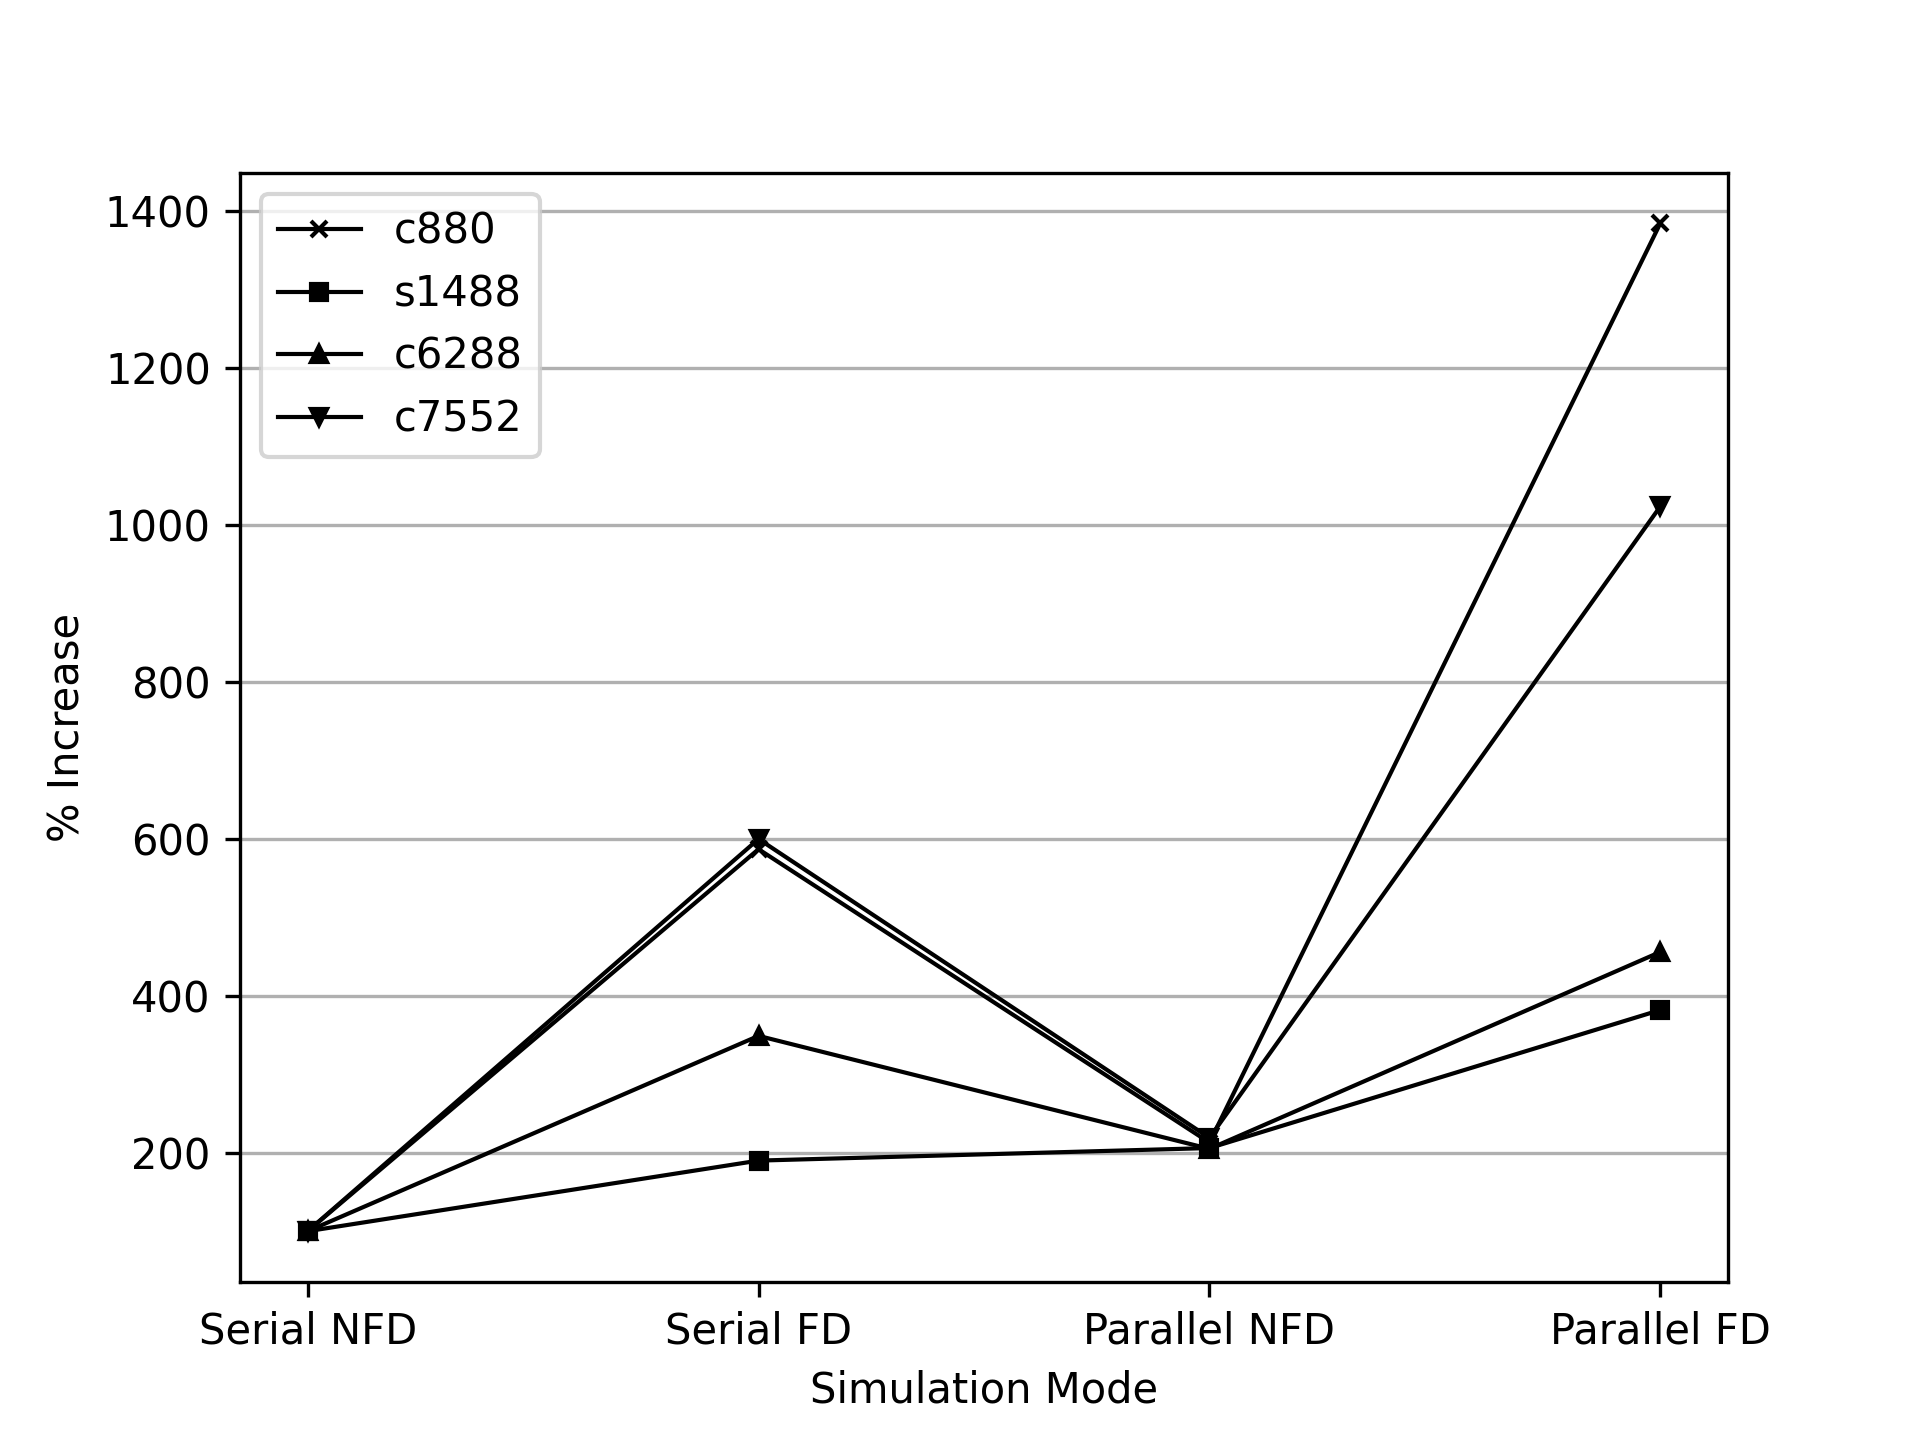
\includegraphics[width=0.7\textwidth]{figure.png}
	%\caption{A picture of a gull.}
\end{figure}

\begin{figure}[h]  
  \centering
    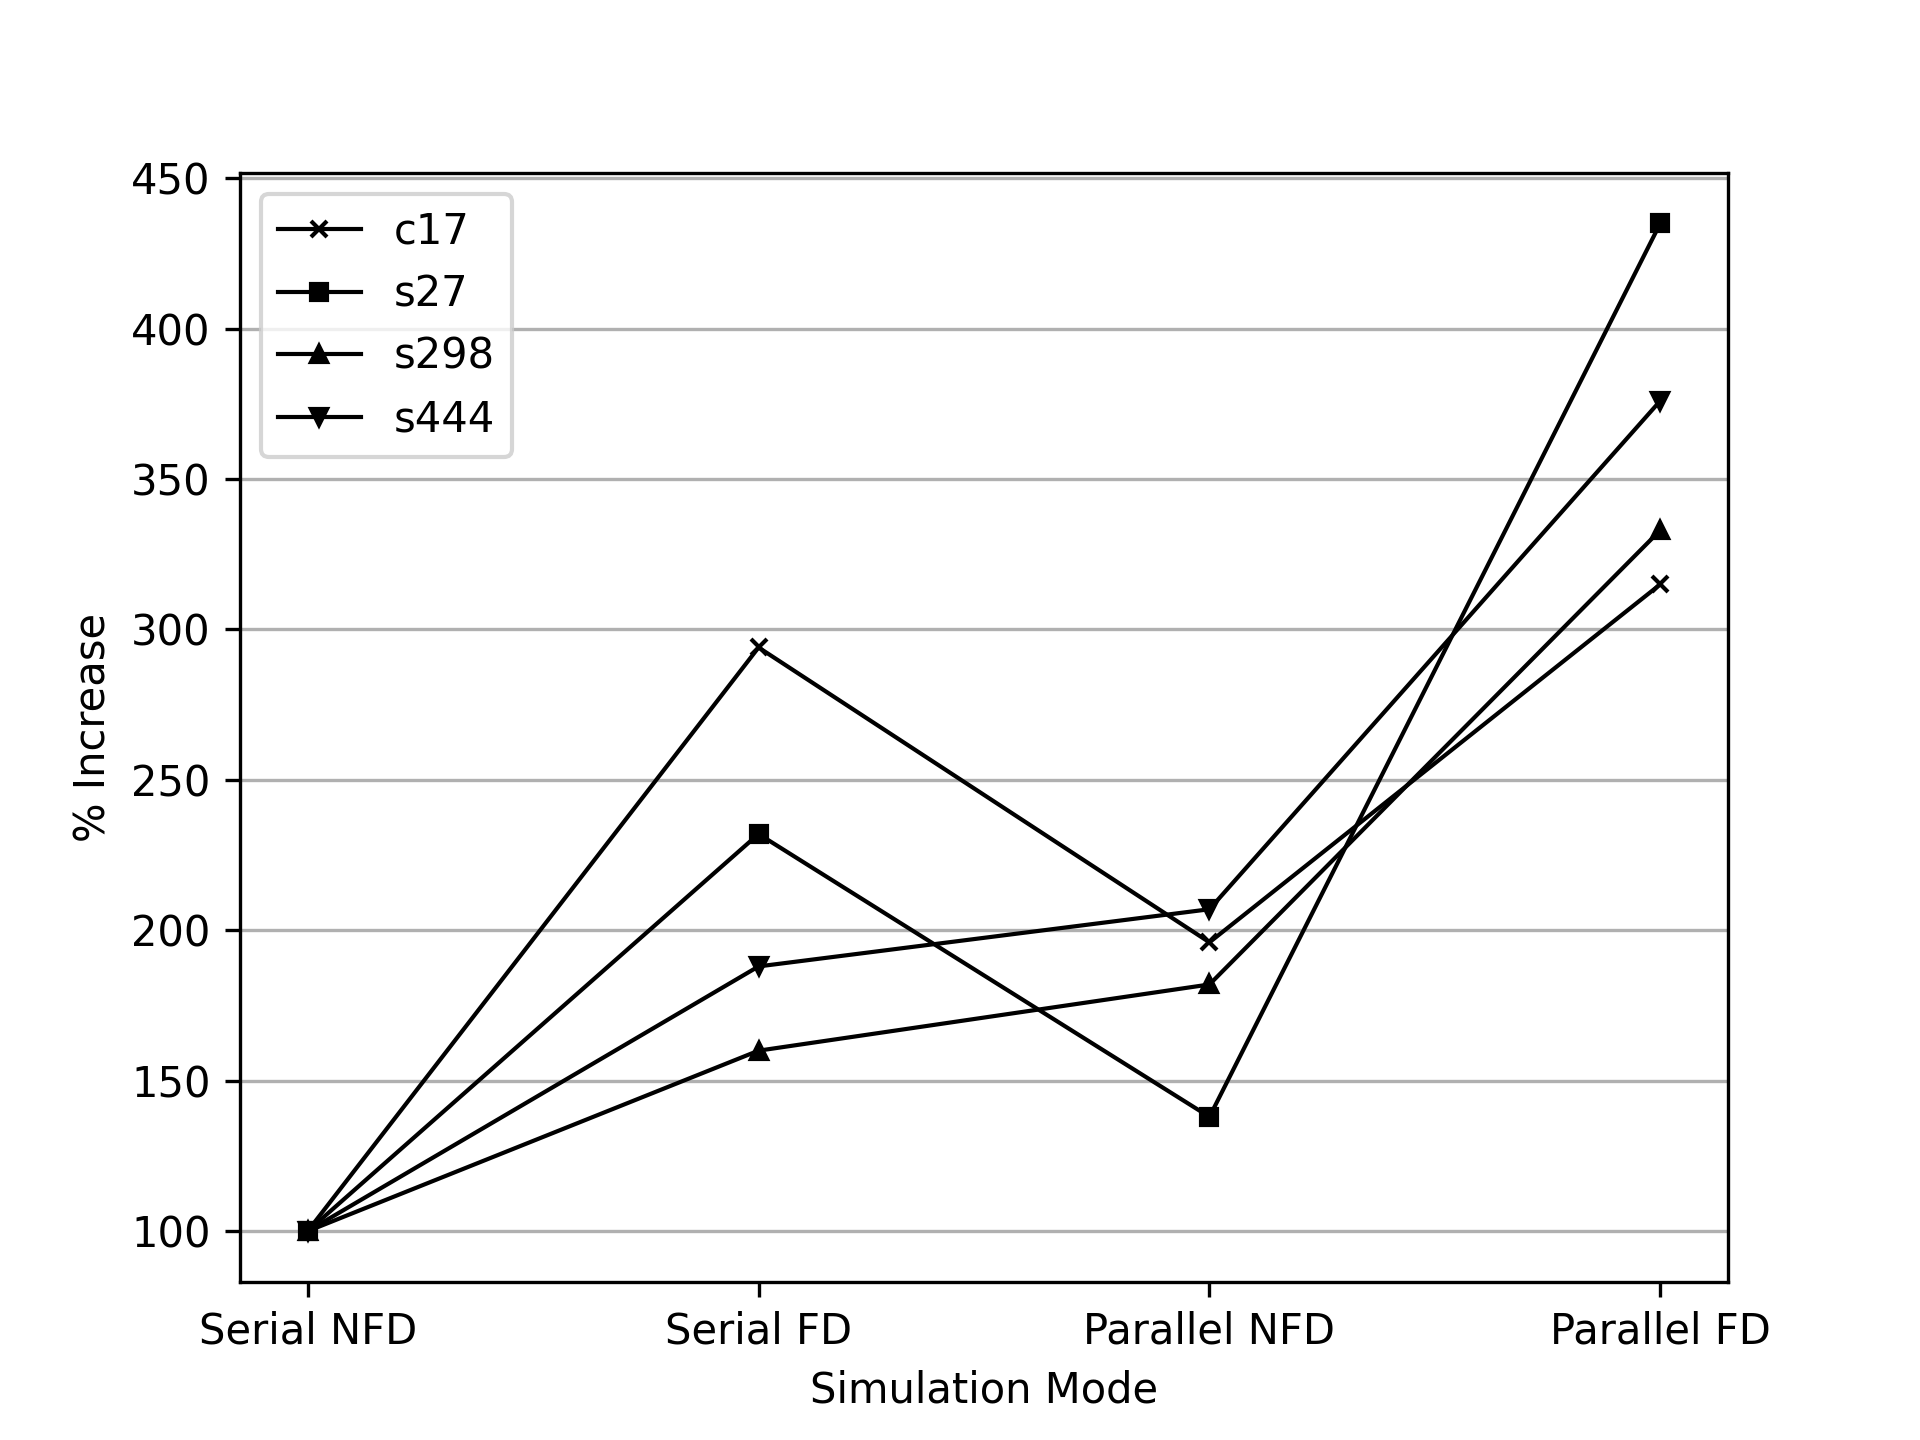
\includegraphics[width=0.7\textwidth]{figure1.png}
	%\caption{A picture of a gull.}
\end{figure}


\begin{figure}[h]  
  \centering
    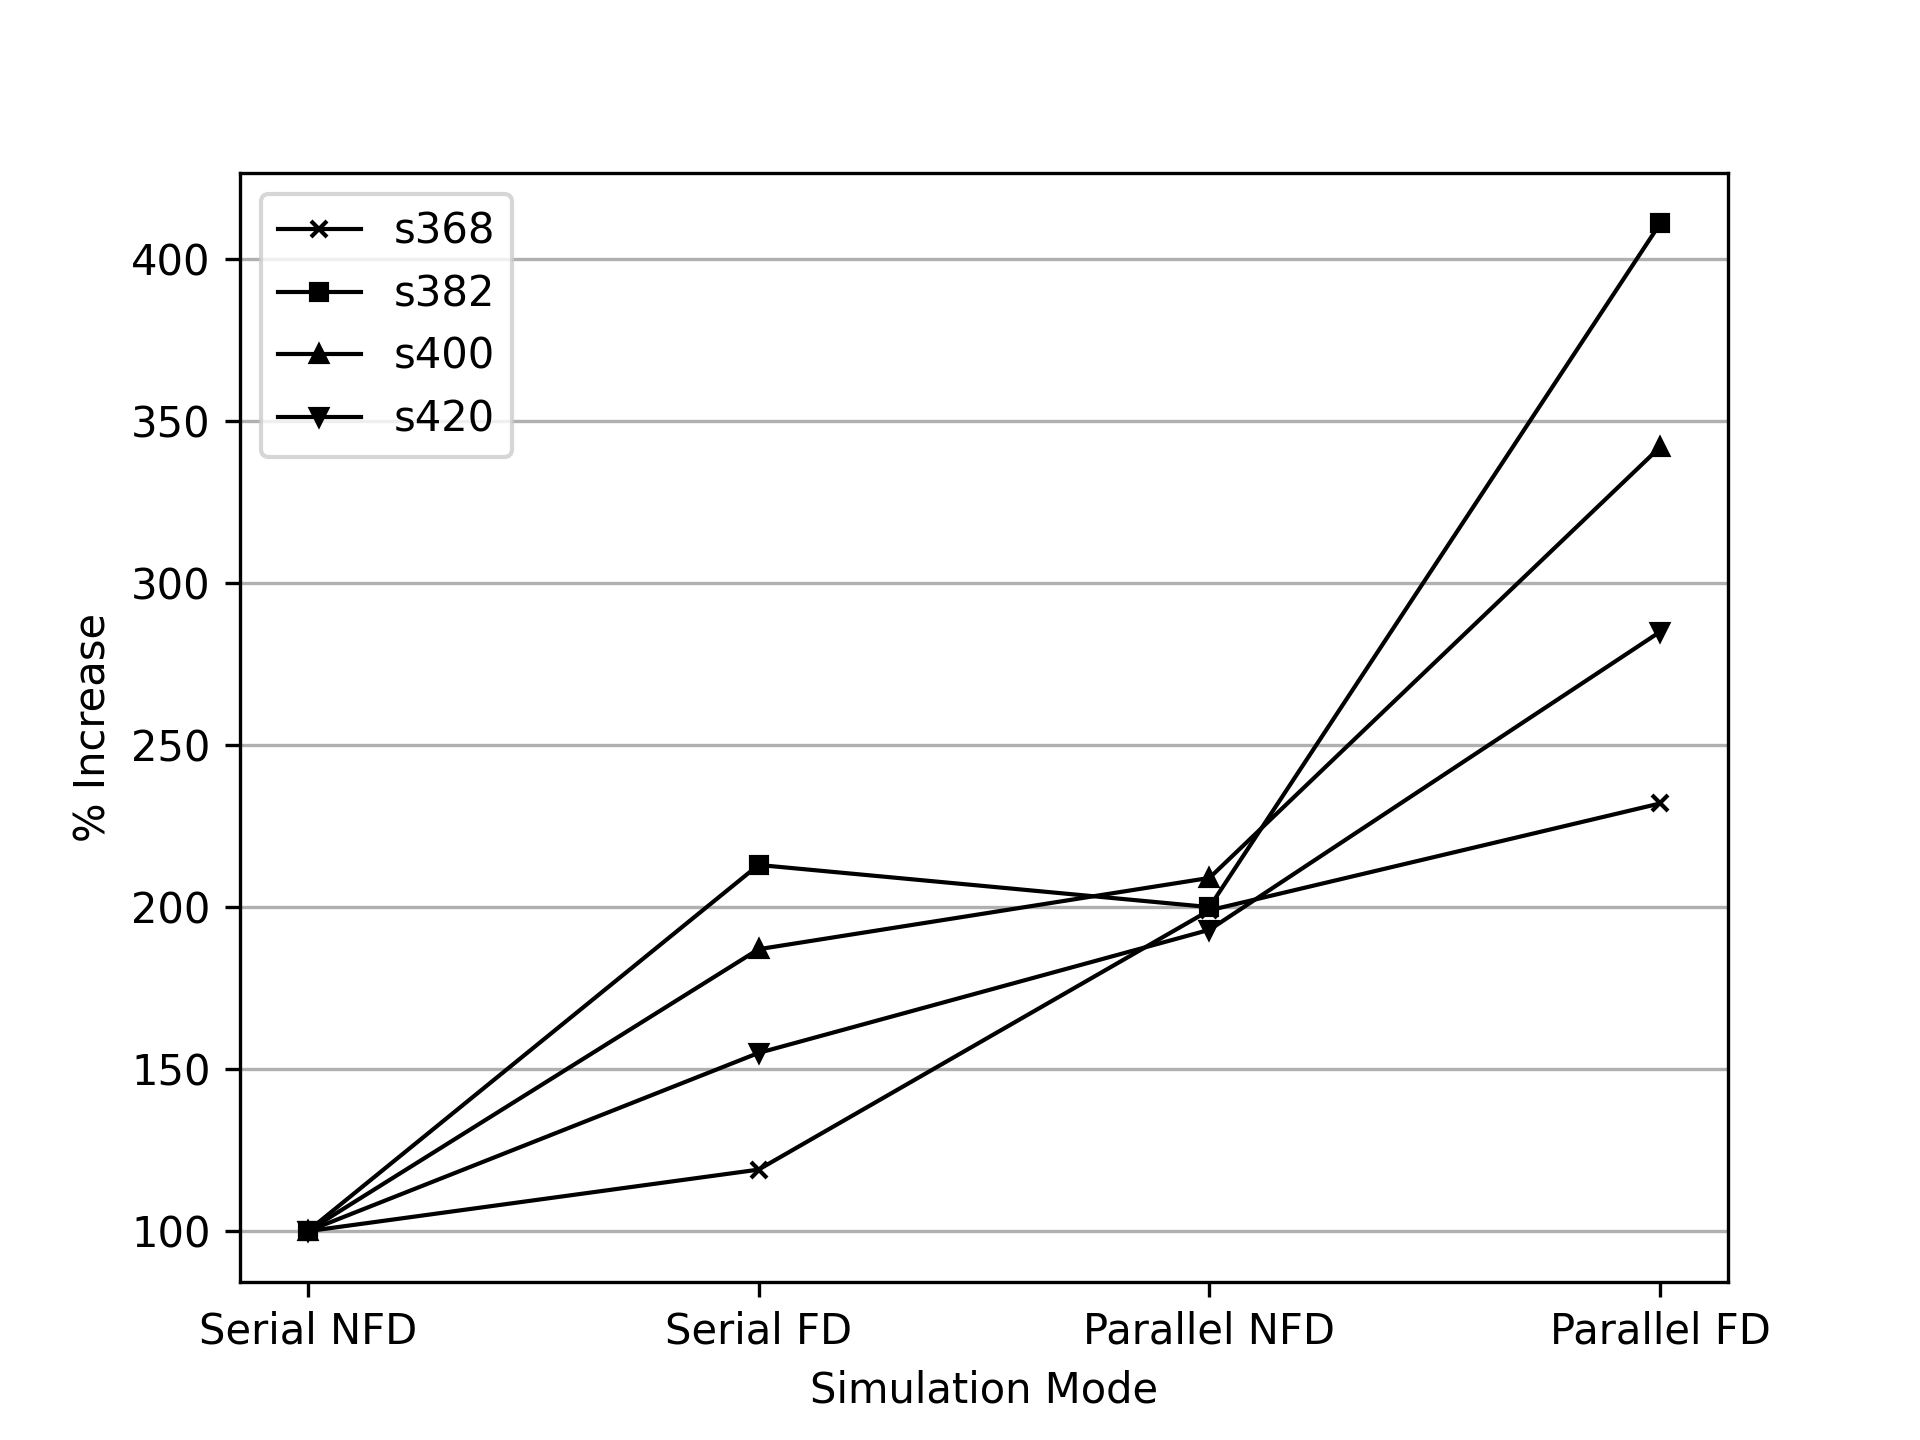
\includegraphics[width=0.7\textwidth]{figure2.png}
	%\caption{A picture of a gull.}
\end{figure}

\begin{figure}[h]  
  \centering
    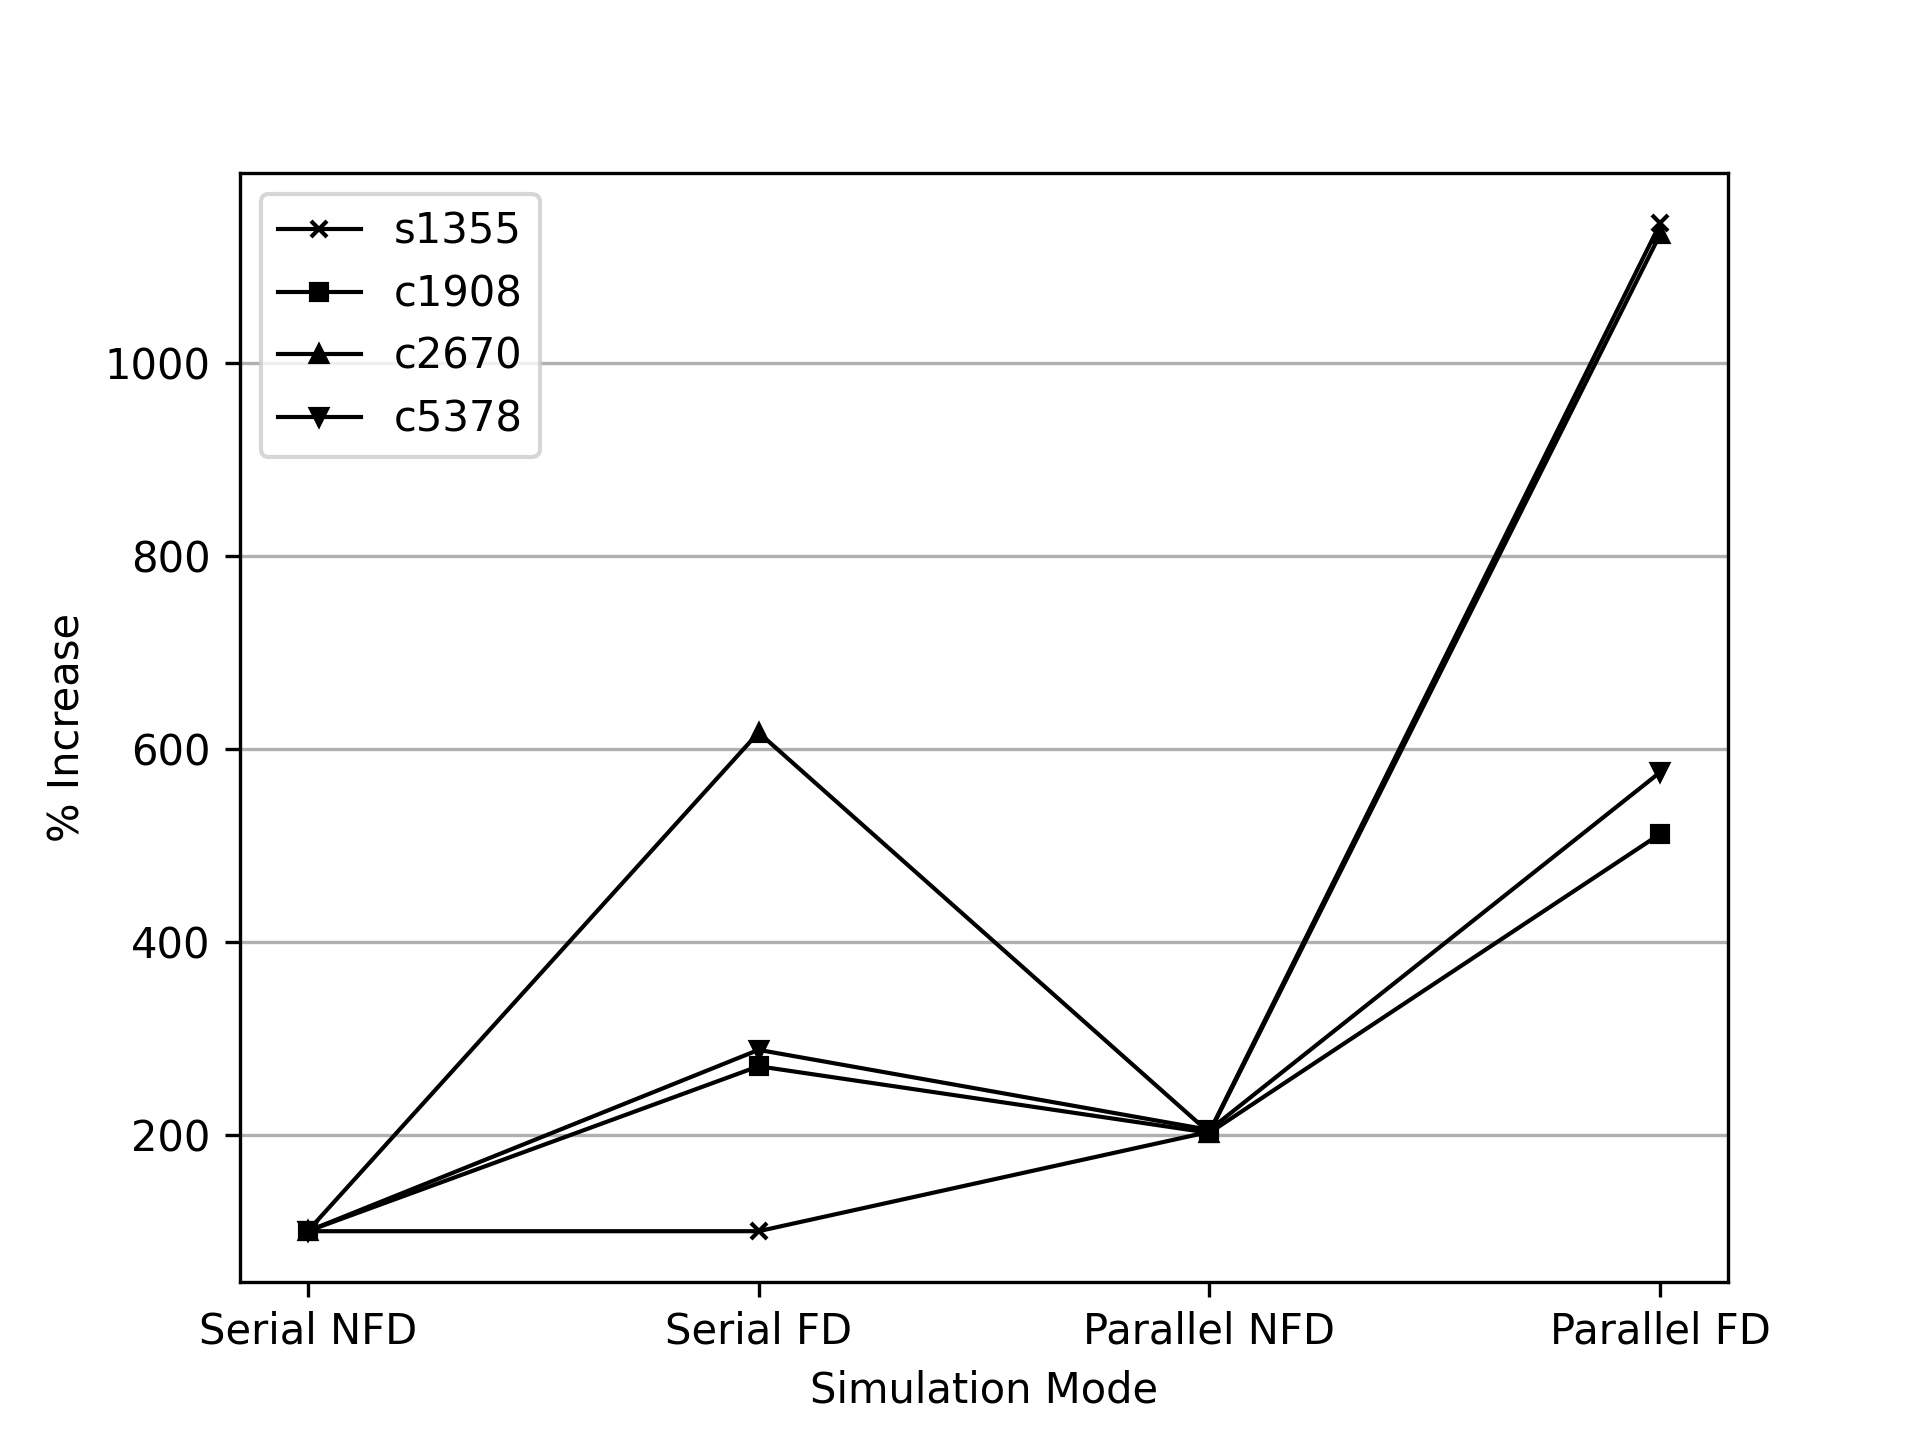
\includegraphics[width=0.7\textwidth]{figure3.png}
	%\caption{A picture of a gull.}
\end{figure}

\clearpage
\section*{Conclusions}
As we can see, the program achieves roughly 200 \% speedup when running in 4 parallel threads compared to running on a single one. Despite not reaching the theoritical maximum of 400 \% a noticable performance increase was observed. Many factors could be limiting the performance increase. One of them is the fact that when a thread detects a single stuck at fault, it accesses a global variable where all detected faults are stored. If the data structure is in use by another thread, then the thread blocks. This is a limiting factor of the current implementation. When looking at the comparison with and without fault dropping a different trend is observed. Specifically, some circuit/test set pairs have a lot more speedup than others. This can be explained by the fact that the potential performance increase depends solely on how good each test set is at detecting stuck at faults. Finally, when looking at the results obtained with the random test vectors, we can clearly see that indeed, just as expected, the fault coverage is roughtly between 60\% - 90\%.

\iffalse
\begin{algorithm}
	\caption{Bruteforce Reliability} 
	\begin{algorithmic}[1]
		\State C = getComponentNumber()
		\State S = getSeconds()
		\State G [ ] = randGraph($|C|$)
		\State T[ ] = getTimesteps($|S|$)
		\State R = 0
		\State N = $2^{|C|}$
		\State Result[ ]
		\For {t in T [ ]}
			\For {i = 0 to N}
				\If {isPath(G)}
					\State R = R + calcReliability(i,t)
				\Else
					\State R = R + 0
				\EndIf	
			\EndFor
		\State Result.append(R,t)
		\EndFor
		
		\State \textbf{return} Result
	\end{algorithmic} 
\end{algorithm}


\begin{algorithm}
	\caption{Upper Bound Approximation} 
	\begin{algorithmic}[1]
		\State C = getComponentNumber()
		\State S = getSeconds()
		\State G [ ] = randGraph($|C|$)
		\State T[ ] = getTimesteps($|S|$)
		\State R = 1
		\State N = $2^{|C|}$
		\State Result[ ]
		\State Paths[ ] = getAllpaths(G)
		\For {t in T [ ]}
			\For {path in Paths[ ]}
				\State R = R $\cdot$ calcReliability(t) 
			\EndFor
		\State Result.append(1-R,t)
		\EndFor
		
		\State \textbf{return} Result
	\end{algorithmic} 
\end{algorithm}


\begin{algorithm}
	\caption{Lower Bound Approximation} 
	\begin{algorithmic}[1]
		\State C = getComponentNumber()
		\State S = getSeconds()
		\State G [ ] = randGraph($|C|$)
		\State T[ ] = getTimesteps($|S|$)
		\State R = 0
		\State N = $2^{|C|}$
		\State Result[ ]
		\State Paths[ ] = getAllpaths(G)
		\For {t in T [ ]}
			\For {path in Paths[ ]}
				\State R = R + calcReliability(t) 
			\EndFor
		\State Result.append($\frac{R}{|Paths|}$,t)
		\EndFor
		
		\State \textbf{return} Result
	\end{algorithmic} 
\end{algorithm}
\fi

\end{document}
